
%=======================   Default Templete   ==================
\documentclass[a4paper]{article}


% file with some default definations
%%%%%%%%%%%%%%%%%%%%%%%%%%%%%%%%%%%%%%%%%
% Lachaise Assignment
% Structure Specification File
% Version 1.0 (26/6/2018)
%
% This template originates from:
% http://www.LaTeXTemplates.com
%
% Authors:
% Marion Lachaise & François Févotte
% Vel (vel@LaTeXTemplates.com)
%
% License:
% CC BY-NC-SA 3.0 (http://creativecommons.org/licenses/by-nc-sa/3.0/)
% 
%%%%%%%%%%%%%%%%%%%%%%%%%%%%%%%%%%%%%%%%%

%----------------------------------------------------------------------------------------
%	PACKAGES AND OTHER DOCUMENT CONFIGURATIONS
%----------------------------------------------------------------------------------------

\usepackage{amsmath,amsfonts,stmaryrd,amssymb} % Math packages

\usepackage{amsthm}

\usepackage{enumerate} % Custom item numbers for enumerations

\usepackage[ruled]{algorithm2e} % Algorithms

\usepackage[framemethod=tikz]{mdframed} % Allows defining custom boxed/framed environments

\usepackage{listings} % File listings, with syntax highlighting
\lstset{
	basicstyle=\ttfamily, % Typeset listings in monospace font
}

%----------------------------------------------------------------------------------------
%	DOCUMENT MARGINS
%----------------------------------------------------------------------------------------

\usepackage{geometry} % Required for adjusting page dimensions and margins

\geometry{
	paper=a4paper, % Paper size, change to letterpaper for US letter size
	top=2.5cm, % Top margin
	bottom=3cm, % Bottom margin
	left=2.5cm, % Left margin
	right=2.5cm, % Right margin
	headheight=14pt, % Header height
	footskip=1.5cm, % Space from the bottom margin to the baseline of the footer
	headsep=1.2cm, % Space from the top margin to the baseline of the header
	%showframe, % Uncomment to show how the type block is set on the page
}

%----------------------------------------------------------------------------------------
%	FONTS
%----------------------------------------------------------------------------------------

\usepackage[utf8]{inputenc} % Required for inputting international characters
\usepackage[T1]{fontenc} % Output font encoding for international characters

\usepackage{XCharter} % Use the XCharter fonts

%----------------------------------------------------------------------------------------
%	COMMAND LINE ENVIRONMENT
%----------------------------------------------------------------------------------------

% Usage:
% \begin{commandline}
%	\begin{verbatim}
%		$ ls
%		
%		Applications	Desktop	...
%	\end{verbatim}
% \end{commandline}

\mdfdefinestyle{commandline}{
	leftmargin=10pt,
	rightmargin=10pt,
	innerleftmargin=15pt,
	middlelinecolor=black!50!white,
	middlelinewidth=2pt,
	frametitlerule=false,
	backgroundcolor=black!5!white,
	frametitle={Command Line},
	frametitlefont={\normalfont\sffamily\color{white}\hspace{-1em}},
	frametitlebackgroundcolor=black!50!white,
	nobreak,
}

% Define a custom environment for command-line snapshots
\newenvironment{commandline}{
	\medskip
	\begin{mdframed}[style=commandline]
}{
	\end{mdframed}
	\medskip
}

%----------------------------------------------------------------------------------------
%	FILE CONTENTS ENVIRONMENT
%----------------------------------------------------------------------------------------

% Usage:
% \begin{file}[optional filename, defaults to "File"]
%	File contents, for example, with a listings environment
% \end{file}

\mdfdefinestyle{file}{
	innertopmargin=1.6\baselineskip,
	innerbottommargin=0.8\baselineskip,
	topline=false, bottomline=false,
	leftline=false, rightline=false,
	leftmargin=2cm,
	rightmargin=2cm,
	singleextra={%
		\draw[fill=black!10!white](P)++(0,-1.2em)rectangle(P-|O);
		\node[anchor=north west]
		at(P-|O){\ttfamily\mdfilename};
		%
		\def\l{3em}
		\draw(O-|P)++(-\l,0)--++(\l,\l)--(P)--(P-|O)--(O)--cycle;
		\draw(O-|P)++(-\l,0)--++(0,\l)--++(\l,0);
	},
	nobreak,
}

% Define a custom environment for file contents
\newenvironment{file}[1][File]{ % Set the default filename to "File"
	\medskip
	\newcommand{\mdfilename}{#1}
	\begin{mdframed}[style=file]
}{
	\end{mdframed}
	\medskip
}

%----------------------------------------------------------------------------------------
%	NUMBERED QUESTIONS ENVIRONMENT
%----------------------------------------------------------------------------------------

% Usage:
% \begin{question}[optional title]
%	Question contents
% \end{question}

\mdfdefinestyle{question}{
	innertopmargin=1.2\baselineskip,
	innerbottommargin=0.8\baselineskip,
	roundcorner=5pt,
	nobreak,
	singleextra={%
		\draw(P-|O)node[xshift=1em,anchor=west,fill=white,draw,rounded corners=5pt]{%
		Question \theQuestion\questionTitle};
	},
}

\newcounter{Question} % Stores the current question number that gets iterated with each new question

% Define a custom environment for numbered questions
\newenvironment{question}[1][\unskip]{
	\bigskip
	\stepcounter{Question}
	\newcommand{\questionTitle}{~#1}
	\begin{mdframed}[style=question]
}{
	\end{mdframed}
	\medskip
}

%----------------------------------------------------------------------------------------
%	WARNING TEXT ENVIRONMENT
%----------------------------------------------------------------------------------------

% Usage:
% \begin{warn}[optional title, defaults to "Warning:"]
%	Contents
% \end{warn}

\mdfdefinestyle{warning}{
	topline=false, bottomline=false,
	leftline=false, rightline=false,
	nobreak,
	singleextra={%
		\draw(P-|O)++(-0.5em,0)node(tmp1){};
		\draw(P-|O)++(0.5em,0)node(tmp2){};
		\fill[black,rotate around={45:(P-|O)}](tmp1)rectangle(tmp2);
		\node at(P-|O){\color{white}\scriptsize\bf !};
		\draw[very thick](P-|O)++(0,-1em)--(O);%--(O-|P);
	}
}

% Define a custom environment for warning text
\newenvironment{warn}[1][Warning:]{ % Set the default warning to "Warning:"
	\medskip
	\begin{mdframed}[style=warning]
		\noindent{\textbf{#1}}
}{
	\end{mdframed}
}

%----------------------------------------------------------------------------------------
%	INFORMATION ENVIRONMENT
%----------------------------------------------------------------------------------------

% Usage:
% \begin{info}[optional title, defaults to "Info:"]
% 	contents
% 	\end{info}

\mdfdefinestyle{info}{%
	topline=false, bottomline=false,
	leftline=false, rightline=false,
	nobreak,
	singleextra={%
		\fill[black](P-|O)circle[radius=0.4em];
		\node at(P-|O){\color{white}\scriptsize\bf i};
		\draw[very thick](P-|O)++(0,-0.8em)--(O);%--(O-|P);
	}
}

% Define a custom environment for information
\newenvironment{info}[1][Info:]{ % Set the default title to "Info:"
	\medskip
	\begin{mdframed}[style=info]
		\noindent{\textbf{#1}}
}{
	\end{mdframed}
}
\usepackage{listings}
\lstset{language=Python, basicstyle=\normalsize\sffamily\linespread{0.8}, numbers=left, numberstyle=\small, stepnumber=1, numbersep=5pt}
\usepackage{fancyhdr}
\usepackage{tikz}
\usepackage{tikz-qtree}
\usepackage{mathtools}
\DeclarePairedDelimiter{\ceil}{\lceil}{\rceil}

\setlength{\parindent}{0pt}

\pagestyle{fancy}
\fancyhf{}
\lhead{\textbf{\NAME\ (\ANDREWID)}}
\chead{\textbf{Assignment \HWNUM}}
\rhead{\COURSE}

\renewcommand{\qedsymbol}{\rule{0.7em}{0.7em}}

%==================Header details======================
\newcommand\NAME{Raghukul Raman}
\newcommand\ANDREWID{160538}
\newcommand\HWNUM{2}
\newcommand\COURSE{CS731}
%======================================================

% available formatted sections:
% - COMMAND LINE ENVIRONMENT: \begin{commandline} \end{commandline}
% - FILE CONTENTS ENVIRONMENT: \begin{file}[optional filename, defaults to "File"]
% - NUMBERED QUESTIONS ENVIRONMENT: \begin{question}[optional title]
% - WARNING TEXT ENVIRONMENT(can also be used for note): \begin{warn}[optional title, defaults to "Warning:"]
% - INFORMATION ENVIRONMENT(can be used to mention given details): \begin{info}[optional title, defaults to "Info:"]

%===============================================================
\begin{document}
\begin{question}
    \textbf{Hash functions and proofs of work}
\end{question}
Let $H: P \times S \rightarrow \{ 0,1,...2^n-1 \}$ be a collision resistant hash function. \\

Let $H^\prime$ be a new hash function,
$H^\prime : P \times S \rightarrow \{ 0,1,...2^{n^{\prime}}-1 \}$ (where $n^\prime = n+\log(d)$), defined as:
$$H^\prime(p, s) = (num(s) \text{ mod } d) \: | \: H(p, s)$$
Here $num(s)$, denotes the number representation of $s$. In other words the new hash function is
defined by append $H(p, s)$, to modulo of $s$ wrt $d$.

\begin{warn}[Claim $1$:]
    $H^\prime$ is collision resistant hash function.
\end{warn}
\begin{proof}
    Suppose $H^\prime$ is not a collision resistant hash function, ie. its easy to find $x, y$, such that
    $H^\prime(x) = H^\prime(y)$ and $x \ne y$. Which means that last $n$ bits of $H^\prime(x)$
    are same as that of $H^\prime (y)$, or $H(x) = H(y)$. This contradicts or assumption that $H$
    was collision resistant. 
\end{proof}

\begin{warn}[claim $2$:]
    $H^\prime$ is not proof-of-work secure.
\end{warn}
\begin{proof}
    Note that for every puzzle $p \in P$, $H^\prime (p, 0) = (0 \text{ mod } d) \: | \: H(p, 0) < \dfrac{2^{n^\prime}}{d}$. \\

For a fixed difficulty($d$), it's trivial to find a solution, or $H^\prime$ is not proof-of-work secure.
\end{proof}
Therefore, there is a collision resistant hash function that is not proof-of-work secure.

\begin{question}
    \textbf{Beyond binary Merkle trees}
\end{question}
\subsubsection*{(a)}
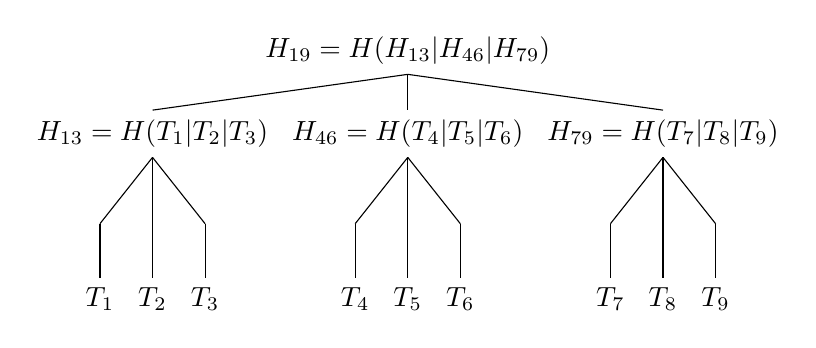
\begin{tikzpicture}
\Tree [.$H_{19}=H(H_{13}|H_{46}|H_{79})$ [.$H_{13}=H(T_1|T_2|T_3)$ [ $T_1$ ] [ $T_2$ ] [ $T_3$ ] ]
                                  [.$H_{46}=H(T_4|T_5|T_6)$ [ $T_4$ ] [ $T_5$ ] [ $T_6$ ] ]
                                  [.$H_{79}=H(T_7|T_8|T_9)$ [ $T_7$ ] [ $T_8$ ] [ $T_9$ ] ]
        ]
\end{tikzpicture}

Commitment tree for $S=\{ T_1, T_2, ...T_9\}$ \\
Each node of the tree stores the hash of it's $3$ children concatenated. Finally Alice keeps the hash value of
root of merkle tree. \\
To prove membership of $T_4$, Alice need to provide values of $T_5,T_6, H_{13}, H_{79}$. Bob verifies them
by computing $H_{46}$ using $T_4, T_5, T_6$, and then computes $H_{19}$ using computes $H_{46}$ and provided
$H_{13}, H_{79}$, and compare with the root hash stored earlier.

\subsubsection*{(b)}
Note that height of above merkle tree as a function of $n, k$ is $\ceil{\log_k n}$
For each level we need to store $k-1$ for proof.\\
Length of proof to prove existance of $T_i$ is $(k-1)\ceil{\log_k n}$, in above example it is $2\ceil{\log_3 n}$

\subsubsection*{(c)}
In a binary tree $k = 2$, ie proof size = $\ceil{\log n}$, while for a general k-ary tree it is $(k-1)\ceil{\log_k n}$ \\

Their ratio is:
$$\dfrac{(k-1)\ceil{\log_k n}}{\ceil{\log n}}$$
ignoring the ceil function we get:
$$\dfrac{(k-1)\log_k n}{\log n} =  \dfrac{(k-1)\log 2}{\log k} >> 1 \text{ as $k$ increases}$$
One advantage of this over the regular binary merkle tree can be that we would need to compute very few hash
, ie this would be beneficial for constly hash functions.
Precisely we need to call $H$ $\ceil{\log_k n}$ times, which is approximately $\log k$ times better
that binary tree.

\begin{question}
    \textbf{Hiding vs. binding commitments}
\end{question}

\subsubsection*{(a)}
Assuming $10$ digit phone numbers there can be atmost $10^{10}$ valid phone numbers. Bob can precompute the 
hash of all these valid phone numbers, and create a hashmap of hash value to mobile number.
Whenever a new user registers, he just checks his/her phone number from the hashmap, he can do the
same thing for the contacts of this user. Hence Bob can act maliciously to determine the phone
numbers and contacts of all BobCrypt users.


\subsubsection*{(b)}
Using a $128$ bit nounce will not work since then it would not be possible to add friends on the app.
Let's say $B$ creates a new account, and $B$ has $A's$ contact number in his phone, but since the
does not store the nounce explicity, $B$ will not be able to add $A$ just using his phone number. Hence
BobCrypt $2.0$ will not be able to provide intended functionality.

\begin{question}
    \textbf{Bitcoin script}
\end{question}



\begin{question}
    \textbf{Lightweight clients}
\end{question}

\subsubsection*{(a)}
Since Bob only has the header of last block of blockchain, Alice needs to send the merkle tree proof 
of the block in which this transaction is present. Along with merkle tree proof, she also need to 
send the all the block headers from the second most recent block to the one having this transaction. \\

To check Bob will verify merkle tree existance using the proof provided, compute block hashes consequtively
and then finally verify the block hash with current block header's previous block field.

\subsubsection*{(b)}
\begin{align*}
   \text{Proof size} &= \text{Block headers +  Merkle Proof} \\
    &= k*size\_of(\text{block\_header}) + \ceil{\log n}*size\_of(\text{one merkle proof unit})
\end{align*}

\subsubsection*{(c)}

\begin{question}
    \textbf{BitcoinLotto}
\end{question}
\subsubsection*{(a)}
To prevent the winner from spending money on first we can implement a $2$  of $2$ multisig. In other words,
the winner has a private key, but to use the money, transaction must be signed by trusted printing factory
(who have the other private key) and the winner. Private key of winner is implemented using 2-of-2 multisig.

\subsubsection*{(b)}
To prevent loss of lost ticket's money, we can make a transaction with locktime of $1$ week to the next week's
address. If the ticket is lost, the money will automatically go to the next week's lottery.


\end{document}
